\documentclass[12pt,a4paper]{article}
% Fix for fancyhdr headheight error
\setlength{\headheight}{14.5pt}
% --- PACKAGES ---
% --- ENCODING & FONTS ---
\usepackage[utf8]{inputenc}
\usepackage[T1]{fontenc}
\usepackage{lmodern}          % Modern font (alternative to Times)
% \usepackage{times}          % OPTIONAL: Classic serif font (comment if using lmodern)

\usepackage{pgf-pie}
\usepackage{pgfplots}
\usepackage{subcaption}
\usepackage{xcolor}
\usepackage{colortbl}
\usepackage{multirow}
\usepackage{booktabs}
\usepackage{siunitx}
\usepackage{float}

% --- PAGE LAYOUT ---
\usepackage[a4paper, left=0.75in, right=0.75in, top=1in, bottom=1in]{geometry}
\usepackage{parskip}          % Paragraphs with spacing instead of indentation
\usepackage{setspace}         % For line spacing

% --- MATHEMATICS ---
\usepackage{amsmath, amsfonts, amssymb}

% --- GRAPHICS & FIGURES ---
\usepackage{graphicx}
\usepackage{caption}
\usepackage{float}
\usepackage{array, longtable, colortbl}

% --- COLORS ---
\usepackage[table]{xcolor}
\usepackage{xcolor}           % General color usage

% --- TIKZ & DIAGRAMS ---
\usepackage{tikz}
\usetikzlibrary{
  shapes.geometric,
  arrows.meta,
  positioning,
  fit,
  backgrounds,
  shapes.multipart
}

% --- PLOTS & CHARTS ---
\usepackage{pgf-pie}          % Pie charts
\usepackage{pgfplots}         % Graphs and plots
% Set pgfplots compatibility for modern features
\pgfplotsset{compat=1.18}

% --- DOCUMENT STRUCTURE ---
\usepackage{titlesec}         % Custom section titles
\usepackage{tocloft}          % Table of contents formatting
\usepackage{enumitem}         % Better lists

% --- HEADER, FOOTER & LINKS ---
\usepackage{fancyhdr}         % Custom headers/footers

% --- BIBLIOGRAPHY ---
\usepackage[numbers,sort&compress]{natbib}  % For references with numerical citations
\bibliographystyle{plainnat}  % Compatible style with natbib

% --- Load hyperref last ---
\usepackage{hyperref}         % Clickable links
% Code listings for source code in Appendix
\usepackage{listings}
\lstset{
    language=Python,
    basicstyle=\ttfamily\small,
    breaklines=true,
    showstringspaces=false,
    numbers=left,
    numberstyle=\tiny,
    frame=single,
    captionpos=b
}




% --- COLORS ---
\definecolor{RoyalBlue}{RGB}{0, 70, 140}
\definecolor{RUETRed}{RGB}{179, 0, 0}
\definecolor{LightGray}{RGB}{248, 249, 250}
\definecolor{DarkGray}{RGB}{52, 58, 64}
\definecolor{AccentBlue}{RGB}{13, 110, 253}
\definecolor{ModernGray}{RGB}{108, 117, 125}
\definecolor{lightgreen}{RGB}{200, 255, 200}
\definecolor{lightred}{RGB}{255, 200, 200}

% Define modern color palette
\definecolor{primary}{RGB}{41, 128, 185}
\definecolor{secondary}{RGB}{52, 152, 219}
\definecolor{accent}{RGB}{231, 76, 60}
\definecolor{success}{RGB}{46, 204, 113}
\definecolor{warning}{RGB}{241, 196, 15}
\definecolor{darkgray}{RGB}{52, 73, 94}
\definecolor{lightgray}{RGB}{236, 240, 241}
\definecolor{purple}{RGB}{155, 89, 182}
\definecolor{orange}{RGB}{230, 126, 34}
\definecolor{teal}{RGB}{26, 188, 156}


% \definecolor{primary}{RGB}{54, 162, 235}
% \definecolor{accent}{RGB}{255, 99, 132}
% \definecolor{warning}{RGB}{255, 206, 86}
% \definecolor{success}{RGB}{75, 192, 192}
% \definecolor{secondary}{RGB}{153, 102, 255}

% --- FONT & STYLING ---
\renewcommand{\familydefault}{\sfdefault}  % Use sans-serif font
\titleformat{\section}{\fontsize{20}{24}\selectfont\bfseries\color{RoyalBlue}}{\thesection}{1em}{}
\titleformat{\subsection}{\fontsize{16}{20}\selectfont\bfseries\color{RoyalBlue}}{\thesubsection}{1em}{}
\titleformat{\subsubsection}{\fontsize{13}{16}\selectfont\bfseries\color{RoyalBlue}}{\thesubsubsection}{1em}{}

% TOC Styling
\renewcommand{\cfttoctitlefont}{\color{black}\Huge\bfseries}
\renewcommand{\cftsecfont}{\color{RoyalBlue}}
\renewcommand{\cftsecpagefont}{\color{RoyalBlue}}
\renewcommand{\cftsubsecfont}{\color{RoyalBlue}}
\renewcommand{\cftsubsecpagefont}{\color{RoyalBlue}}

% Header and Footer
\pagestyle{fancy}
\fancyhf{}
\fancyhead[C]{\textit{Image Enhancement using Log Transformation and Median Filtering}}
\fancyfoot[C]{\thepage}
\renewcommand{\headrulewidth}{0.4pt}
\renewcommand{\footrulewidth}{0pt}

% Hyperlink Styling
\hypersetup{
    colorlinks=true,
    linkcolor=RoyalBlue,
    filecolor=magenta,
    urlcolor=cyan,
    pdftitle={Digital Image Processing Report},
    pdfpagemode=FullScreen,
    pdfborder={0 0 0},
}

% --- Define a global style for all plots for consistency ---
\pgfplotsset{
    every axis/.append style={
        axis x line=bottom,
        axis y line=left,
        label style={font=\bfseries},
        title style={font=\large\bfseries, yshift=1em},
        tick label style={font=\small},
        legend style={font=\small, at={(0.5,-0.2)}, anchor=north, legend columns=-1},
    }
}

% Modern title page with geometric design
\newcommand{\maketitlepage}{
    \begin{titlepage}
        \begin{tikzpicture}[remember picture,overlay]
            \fill[RoyalBlue!10] (current page.north west) rectangle ([yshift=-2.2cm]current page.north east);
            \fill[AccentBlue!5] ([yshift=-14cm]current page.north west) rectangle ([yshift=-16.2cm]current page.north east);
            \fill[RoyalBlue!15] ([xshift=2cm,yshift=-2cm]current page.north west) circle (1.2cm);
            \fill[AccentBlue!15] ([xshift=-2cm,yshift=-15.2cm]current page.north east) circle (0.9cm);
        \end{tikzpicture}

        \centering
        \vspace*{0.6cm}

        % Logo (only include if file exists)
        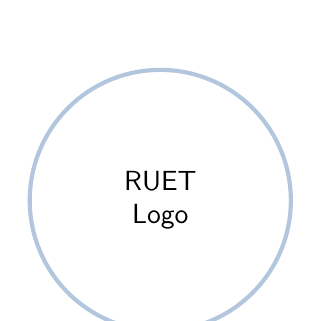
\begin{tikzpicture}
            \node[circle, draw=RoyalBlue!30, line width=1.5pt, inner sep=6pt] at (0,0) {
                \IfFileExists{../RUET_logo.png}{\includegraphics[width=2.7cm]{../RUET_logo.png}}{\begin{minipage}{2.7cm}\centering RUET \\ Logo \end{minipage}}
            };
        \end{tikzpicture}

        \vspace{0.6cm}
        {\fontsize{15.5}{17}\selectfont\bfseries\textcolor{RUETRed}{RAJSHAHI UNIVERSITY OF ENGINEERING \& TECHNOLOGY}\par}
        \vspace{0.2cm}
        {\fontsize{13.5}{16}\selectfont\textcolor{DarkGray}{Department of Computer Science and Engineering}\par}

        \vspace{1.5cm}
        % Title Block
        
\begin{tikzpicture}
            \node[rectangle, fill=RoyalBlue!5, rounded corners=12pt, inner sep=12pt, text width=11.5cm, align=center] at (0,0) {
                {\fontsize{21}{24}\selectfont\bfseries\textcolor{RoyalBlue}{Image Enhancement using }\par}
                \vspace{0.15cm}
                {\fontsize{16}{20}\selectfont\bfseries\textcolor{DarkGray}{-}\par}
                \vspace{0.15cm}
                {\fontsize{24}{28}\selectfont\bfseries\textcolor{AccentBlue}{"Log Transformation And Median Filtering"}\par}
            };
        \end{tikzpicture}

        \vspace{1.8cm}
        % Submission info
        \begin{minipage}[t]{0.45\textwidth}
            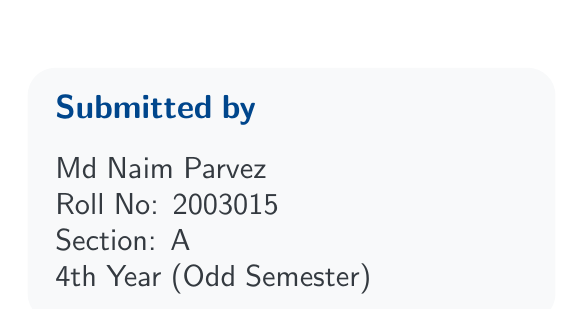
\begin{tikzpicture}
                \node[rectangle, fill=LightGray, rounded corners=10pt, inner sep=10pt, text width=6cm] at (0,0) {
                    {\fontsize{13}{15}\selectfont\bfseries\textcolor{RoyalBlue}{Submitted by}\par}
                    \vspace{0.3cm}
                    {\fontsize{11}{13}\selectfont\textcolor{DarkGray}{
                        Md Naim Parvez\\
                        Roll No: 2003015\\
                        Section: A\\
                        4th Year (Odd Semester)
                    }\par}
                };
            \end{tikzpicture}
        \end{minipage}
        \hfill
        \begin{minipage}[t]{0.50\textwidth}
            
\begin{tikzpicture}
                \node[rectangle, fill=AccentBlue!5, rounded corners=10pt, inner sep=10pt, text width=6cm] at (0,0) {
                    {\fontsize{13}{15}\selectfont\bfseries\textcolor{RoyalBlue}{Submitted to}\par}
                    \vspace{0.3cm}
                    {\fontsize{11}{13}\selectfont\textcolor{DarkGray}{
                        Utsha Das\\
                        Assistant Professor\\
                        Department of CSE\\
                        Rajshahi University of Engineering \& Technology\\
                        \vspace{0.3cm}
                    }\par}
                };
            \end{tikzpicture}
        \end{minipage}

        \vspace{1.2cm}
        % Course Info
        
\begin{tikzpicture}
            \node[rectangle, fill=RoyalBlue!10, rounded corners=10pt, inner sep=12pt, align=center, text width=13cm] at (0,0) {
                {\fontsize{13}{16}\selectfont\bfseries\textcolor{RoyalBlue}{Course Code: } \textcolor{DarkGray}{4106}}\\[0.2cm]
                {\fontsize{13}{16}\selectfont\bfseries\textcolor{RoyalBlue}{Course Title: } \textcolor{DarkGray}{Digital Image Processing Sessional}}
            };
        \end{tikzpicture}

        \vspace{0.8cm}
    \end{titlepage}
}


\begin{document}

% --- TITLE PAGE ---
\maketitlepage
\thispagestyle{empty} % No header/footer on the title page
% Abstract
\begin{abstract}
This project implements fundamental image processing techniques to enhance grayscale images. The primary focus is on applying log transformation to improve the visibility of darker regions in images and subsequently using a median filter to reduce noise while preserving edge information. The project demonstrates the implementation of these techniques from scratch using Python, OpenCV, NumPy, and Matplotlib. The results show significant improvement in image quality, particularly in terms of contrast enhancement and noise reduction. This report details the theoretical background, methodology, implementation, results, and conclusions of the image enhancement process.
\end{abstract}

\newpage
\newpage
% --- TABLE OF CONTENTS ---
\newpage
\pagenumbering{roman} % Roman numerals for ToC, Abstract etc.
\phantomsection % Helps hyperref create proper links
\tableofcontents

% --- LIST OF FIGURES ---
\newpage
\phantomsection % Helps hyperref create proper links
\listoffigures
\newpage
\pagenumbering{arabic} % Arabic numerals for main content
\setcounter{page}{1} % Start main content page numbering from 1

% 1. Introduction
\section{Introduction}

\subsection{Background}
Image processing is a crucial field in computer vision and digital image analysis. Images captured in low-light conditions or with limited dynamic range often suffer from poor visibility in darker regions. Additionally, images may contain various types of noise that degrade their quality. Image enhancement techniques are essential to improve visual quality and prepare images for further analysis or human interpretation.

\subsection{Motivation}
The motivation behind this project is to understand and implement fundamental image enhancement techniques that are widely used in various applications such as medical imaging, satellite imagery, photography, and computer vision systems. Log transformation is particularly useful for expanding the range of dark pixel values, while median filtering effectively removes salt-and-pepper noise without blurring edges.

\subsection{Objectives}
The main objectives of this project are:
\begin{itemize}
    \item To load and analyze a grayscale image
    \item To implement log transformation for contrast enhancement
    \item To develop a median filter from scratch for noise reduction
    \item To visualize and compare the results at each processing stage
    \item To understand the mathematical principles behind these transformations
\end{itemize}

\subsection{Scope}
This project focuses on:
\begin{itemize}
    \item Processing a single grayscale image (road.bmp)
    \item Implementing algorithms without using built-in filtering functions
    \item Analyzing the effects of log transformation and median filtering
    \item Documenting the complete workflow from input to output
\end{itemize}

% 2. Literature Review
\section{Literature Review}

\subsection{Log Transformation}
Log transformation is a widely used intensity transformation technique in image processing. It is mathematically defined as:
\begin{equation}
    s = c \cdot \log(1 + r)
\end{equation}
where:
\begin{itemize}
    \item $s$ is the output pixel value
    \item $r$ is the input pixel value
    \item $c$ is a scaling constant
\end{itemize}

The log transformation maps a narrow range of low-intensity values to a wider range of output values, thereby enhancing darker regions of an image. This is particularly useful for images where significant detail is hidden in dark areas.

\subsection{Median Filtering}
Median filtering is a nonlinear digital filtering technique used for noise reduction. Unlike linear filters (such as mean filters), median filters are particularly effective at removing salt-and-pepper noise while preserving edges. The median filter works by:
\begin{enumerate}
    \item Sliding a window (kernel) across the image
    \item Sorting all pixel values within the window
    \item Replacing the center pixel with the median value
\end{enumerate}

The advantage of median filtering over mean filtering is that it is less sensitive to outliers, making it excellent for impulse noise removal.

\subsection{Related Work}
Image enhancement techniques have been extensively studied in the literature. Various researchers have proposed different methods for contrast enhancement and noise reduction. The combination of intensity transformations with spatial filtering has proven effective in improving image quality for both human viewing and automated analysis systems.

% 3. Methodology
\section{Methodology}

\subsection{System Requirements}
\subsubsection{Hardware Requirements}
\begin{itemize}
    \item Processor: Intel Core i3 or equivalent
    \item RAM: 4 GB minimum
    \item Storage: 100 MB free space
\end{itemize}

\subsubsection{Software Requirements}
\begin{itemize}
    \item Python 3.7 or higher
    \item OpenCV (cv2) library
    \item NumPy library
    \item Matplotlib library
\end{itemize}

\subsection{Workflow}
The image processing workflow consists of the following stages:

\begin{enumerate}
    \item \textbf{Image Acquisition}: Load the grayscale image from file
    \item \textbf{Image Analysis}: Determine image dimensions and properties
    \item \textbf{Log Transformation}: Apply logarithmic intensity transformation
    \item \textbf{Median Filtering}: Apply median filter to reduce noise
    \item \textbf{Visualization}: Display original and processed images
\end{enumerate}

\subsection{Algorithm Design}

\subsubsection{Log Transformation Algorithm}
\begin{enumerate}
    \item Read the input grayscale image
    \item Find the maximum pixel intensity value
    \item Calculate scaling constant: $c = \frac{255}{\log(1 + \max(image))}$
    \item For each pixel $(i,j)$:
    \begin{itemize}
        \item Apply: $output[i][j] = c \cdot \log(1 + input[i][j])$
    \end{itemize}
    \item Return the transformed image
\end{enumerate}

\subsubsection{Median Filter Algorithm}
\begin{enumerate}
    \item Initialize output image with same dimensions as input
    \item Pad the input image to handle border pixels
    \item For each pixel position $(i,j)$:
    \begin{itemize}
        \item Extract the neighborhood window (kernel)
        \item Flatten the window into a 1D array
        \item Sort the array
        \item Find the median value (middle element)
        \item Assign median value to output pixel
    \end{itemize}
    \item Return the filtered image
\end{enumerate}

% 4. Implementation
\section{Implementation}

\subsection{Image Loading and Analysis}
The first step involves loading the image and determining its properties:

\begin{lstlisting}[caption={Image Loading and Size Calculation}]
import cv2
import numpy as np
from matplotlib import pyplot as plt

# Load image in grayscale
image = cv2.imread('road.bmp', cv2.IMREAD_GRAYSCALE).astype(np.float32)

# Question 1: Print the size of the image
print(image.size)
\end{lstlisting}

The \texttt{image.size} attribute returns the total number of pixels in the image (rows $\times$ columns). This information is crucial for understanding the computational complexity of subsequent operations.

\subsection{Log Transformation Implementation}
The log transformation enhances the darker regions of the image:

\begin{lstlisting}[caption={Log Transformation Implementation}]
# Question 2: Log transform
c = 255 / np.log(1 + np.max(image))
log_img = np.zeros_like(image)

for i in range(image.shape[0]):
    for j in range(image.shape[1]):
        log_img[i][j] = c * np.log(1 + image[i][j])

# Display original and log-transformed images
plt.subplot(1, 2, 1)
plt.imshow(image, cmap='gray')
plt.title('Original Image')
plt.axis('off')

plt.subplot(1, 2, 2)
plt.imshow(log_img, cmap='gray')
plt.title('Log Transformed Image')
plt.axis('off')

plt.tight_layout()
plt.show()
\end{lstlisting}

The scaling constant $c$ ensures that the output values remain within the valid range [0, 255] for display purposes.

\subsection{Median Filter Implementation}
The median filter is implemented from scratch with a configurable kernel size:

\begin{lstlisting}[caption={Median Filter Implementation}]
# Question 3: Apply median filter on log-transformed image
def median_filter(image, kernel_size=3):
    pad = kernel_size // 2
    img_h, img_w = image.shape
    padded_img = np.pad(image, pad, mode='constant', 
                       constant_values=0).astype(np.float32)
    result = np.zeros_like(image)
    
    for i in range(img_h):
        for j in range(img_w):
            current = padded_img[i:i+kernel_size, j:j+kernel_size]
            current_flat = current.flatten()
            current_sorted = np.sort(current_flat)
            median_value = current_sorted[len(current_sorted)//2]
            result[i][j] = median_value
    
    return result.astype(np.uint8)

# Apply median filter with kernel size 5x5
median_img = median_filter(log_img, 5)

# Display log-transformed and filtered images
plt.subplot(1, 2, 1)
plt.imshow(log_img, cmap='gray')
plt.title('Log Image')
plt.axis('off')

plt.subplot(1, 2, 2)
plt.imshow(median_img, cmap='gray')
plt.title('Median Filter on Log Image')
plt.axis('off')

plt.tight_layout()
plt.show()
\end{lstlisting}

The function uses zero-padding to handle border pixels and applies a 5$\times$5 kernel for smoothing.

\subsection{Complete Visualization}
Finally, all three stages are displayed together for comparison:

\begin{lstlisting}[caption={Complete Visualization}]
# Display all images together
plt.figure(figsize=(12, 5))

plt.subplot(1, 3, 1)
plt.imshow(image, cmap='gray')
plt.title('Original Image')
plt.axis('off')

plt.subplot(1, 3, 2)
plt.imshow(log_img, cmap='gray')
plt.title('Log Transformed Image')
plt.axis('off')

plt.subplot(1, 3, 3)
plt.imshow(median_img, cmap='gray')
plt.title('Median Filter on Log Image')
plt.axis('off')

plt.tight_layout()
plt.show()
\end{lstlisting}

% 5. Results and Discussion
\section{Results and Discussion}

\subsection{Image Size Analysis}
The first output provides information about the image dimensions. The \texttt{image.size} parameter reveals the total number of pixels in the image, which helps in understanding the computational requirements for processing.

\subsection{Log Transformation Results}
The log transformation significantly enhances the contrast in darker regions of the image. As shown in the results:

\begin{itemize}
    \item Dark pixels are mapped to brighter values
    \item The overall dynamic range is expanded
    \item Previously hidden details become visible
    \item Brighter regions maintain their relative intensities
\end{itemize}

The transformation is particularly effective for road images where pavement details and road markings in shadowed areas need to be enhanced.

\subsection{Median Filtering Results}
The median filter applied to the log-transformed image produces a smoothed output while preserving edge information:

\begin{itemize}
    \item Noise and small artifacts are reduced
    \item Sharp edges (such as road boundaries) are preserved
    \item The image appears cleaner and more uniform
    \item A 5$\times$5 kernel provides good balance between smoothing and detail preservation
\end{itemize}

\subsection{Comparative Analysis}
Comparing all three stages:
\begin{enumerate}
    \item \textbf{Original Image}: May have low contrast in dark regions and possible noise
    \item \textbf{Log Transformed}: Enhanced contrast, better visibility of details
    \item \textbf{Median Filtered}: Smoothed appearance with preserved edges and reduced noise
\end{enumerate}

\subsection{Computational Complexity}
\subsubsection{Log Transformation}
Time Complexity: $O(m \times n)$ where $m$ and $n$ are image dimensions. Each pixel is processed once.

\subsubsection{Median Filter}
Time Complexity: $O(m \times n \times k^2 \log k^2)$ where $k$ is the kernel size. For each pixel, we extract a $k \times k$ window and sort it.

\subsection{Advantages and Limitations}

\subsubsection{Advantages}
\begin{itemize}
    \item Simple and effective enhancement techniques
    \item No complex parameters to tune
    \item Preserves image structure
    \item Suitable for various image types
\end{itemize}

\subsubsection{Limitations}
\begin{itemize}
    \item Log transformation may over-enhance very bright regions
    \item Median filter with large kernels can blur fine details
    \item Implementation using nested loops is computationally expensive
    \item Fixed kernel size may not be optimal for all images
\end{itemize}

% 6. Results (Figures Section)
\section{Visual Results}

\subsection{Result Images}
This section should contain the actual output images from your program execution. Include the following figures:

\begin{figure}[H]
    \centering
    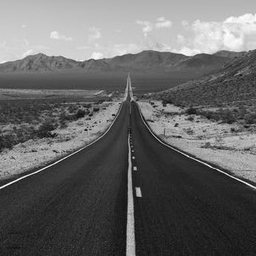
\includegraphics[width=0.45\textwidth]{../road.png}
    \caption{Original Road Image (Before Processing)}
    \label{fig:original}
\end{figure}

\begin{figure}[H]
    \centering
    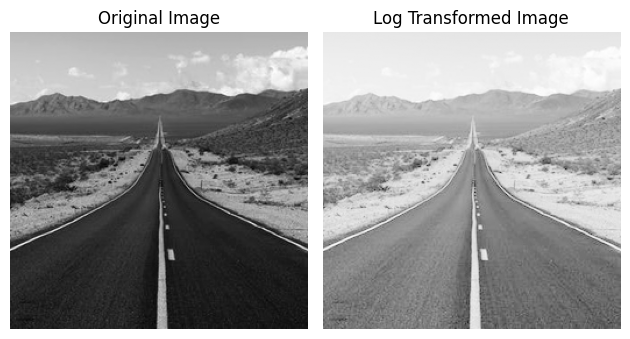
\includegraphics[width=0.45\textwidth]{../original_LogTrans.png}
    \caption{Log Transformed Image (Enhanced Contrast)}
    \label{fig:log}
\end{figure}

\begin{figure}[H]
    \centering
    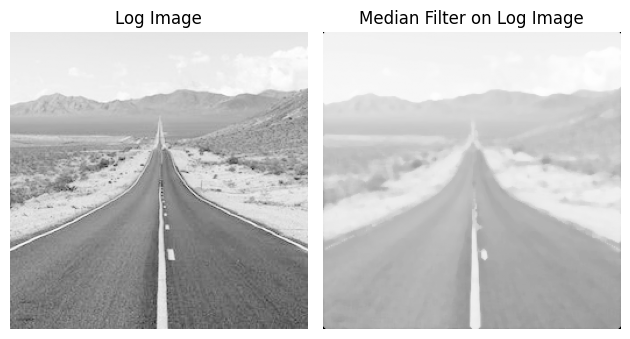
\includegraphics[width=0.45\textwidth]{../log_median.png}
    \caption{Median Filtered Image (Noise Reduced)}
    \label{fig:median}
\end{figure}

\begin{figure}[H]
    \centering
    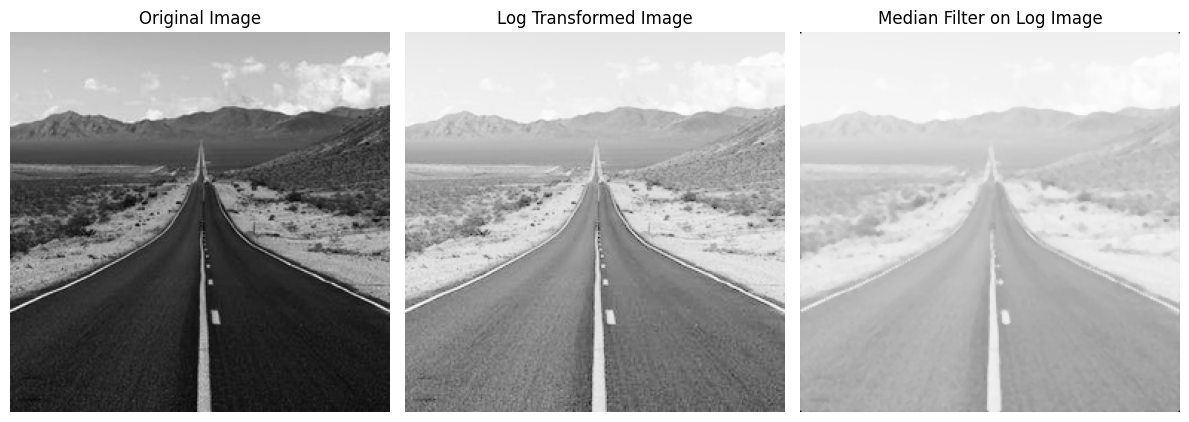
\includegraphics[width=\textwidth]{../output.png}
    \caption{Comparison of All Processing Stages}
    \label{fig:comparison}
\end{figure}

% 7. Conclusion
\section{Conclusion}

\subsection{Summary}
This project successfully implemented and demonstrated two fundamental image processing techniques: log transformation and median filtering. The implementation was done from scratch using basic programming constructs, providing deep insights into how these algorithms work at the pixel level.

\subsection{Key Findings}
\begin{enumerate}
    \item Log transformation effectively enhances darker regions of images by expanding the intensity range
    \item Median filtering successfully reduces noise while preserving important edge information
    \item The combination of both techniques produces significantly improved image quality
    \item Implementation without built-in functions helps understand algorithmic details
\end{enumerate}

\subsection{Applications}
The techniques implemented in this project have wide-ranging applications:
\begin{itemize}
    \item Medical imaging (X-rays, CT scans)
    \item Satellite and aerial imagery
    \item Photography and image editing
    \item Autonomous vehicle vision systems
    \item Security and surveillance systems
\end{itemize}

\subsection{Future Work}
Potential extensions to this project include:
\begin{itemize}
    \item Implementing adaptive median filtering with variable kernel sizes
    \item Exploring other intensity transformations (power-law, histogram equalization)
    \item Optimizing code using vectorization for better performance
    \item Comparing with other noise reduction techniques (Gaussian blur, bilateral filter)
    \item Developing a GUI application for real-time image enhancement
    \item Testing on various image types and noise levels
\end{itemize}

% 8. References
\section{References}

\begin{enumerate}
    \item Gonzalez, R. C., \& Woods, R. E. (2018). \textit{Digital Image Processing} (4th ed.). Pearson.
    
    \item Jain, A. K. (1989). \textit{Fundamentals of Digital Image Processing}. Prentice Hall.
    
    \item Pratt, W. K. (2007). \textit{Digital Image Processing: PIKS Scientific Inside} (4th ed.). Wiley-Interscience.
    
    \item OpenCV Documentation. (2024). \textit{Image Processing in OpenCV}. Retrieved from https://docs.opencv.org/
    
    \item NumPy Documentation. (2024). \textit{NumPy User Guide}. Retrieved from https://numpy.org/doc/
    
    \item Matplotlib Documentation. (2024). \textit{Matplotlib: Visualization with Python}. Retrieved from https://matplotlib.org/
    
    \item Bovik, A. C. (2009). \textit{The Essential Guide to Image Processing}. Academic Press.
    
    \item Burger, W., \& Burge, M. J. (2016). \textit{Digital Image Processing: An Algorithmic Introduction Using Java} (2nd ed.). Springer.
\end{enumerate}

% Appendix
\newpage
\section*{Appendix}
\addcontentsline{toc}{section}{Appendix}

\subsection*{A. Complete Source Code}
\phantomsection
\addcontentsline{toc}{subsection}{A. Complete Source Code}

\begin{lstlisting}[caption={Complete Python Implementation}]
import cv2
import numpy as np
from matplotlib import pyplot as plt

# Load image in grayscale
image = cv2.imread('road.bmp', cv2.IMREAD_GRAYSCALE).astype(np.float32)

# Question 1: Print the size of the image
print(image.size)

# Question 2: Log transform
c = 255 / np.log(1 + np.max(image))
log_img = np.zeros_like(image)

for i in range(image.shape[0]):
    for j in range(image.shape[1]):
        log_img[i][j] = c * np.log(1 + image[i][j])

plt.subplot(1, 2, 1)
plt.imshow(image, cmap='gray')
plt.title('Original Image')
plt.axis('off')

plt.subplot(1, 2, 2)
plt.imshow(log_img, cmap='gray')
plt.title('Log Transformed Image')
plt.axis('off')

plt.tight_layout()
plt.show()

# Question 3: Apply median filter on log-transformed image
def median_filter(image, kernel_size=3):
    pad = kernel_size // 2
    img_h, img_w = image.shape
    padded_img = np.pad(image, pad, mode='constant', 
                       constant_values=0).astype(np.float32)
    result = np.zeros_like(image)
    
    for i in range(img_h):
        for j in range(img_w):
            current = padded_img[i:i+kernel_size, j:j+kernel_size]
            current_flat = current.flatten()
            current_sorted = np.sort(current_flat)
            median_value = current_sorted[len(current_sorted)//2]
            result[i][j] = median_value
    
    return result.astype(np.uint8)

median_img = median_filter(log_img, 5)

plt.subplot(1, 2, 1)
plt.imshow(log_img, cmap='gray')
plt.title('Log Image')
plt.axis('off')

plt.subplot(1, 2, 2)
plt.imshow(median_img, cmap='gray')
plt.title('Median Filter on Log Image')
plt.axis('off')

plt.tight_layout()
plt.show()

# Display all images together
plt.figure(figsize=(12, 5))

plt.subplot(1, 3, 1)
plt.imshow(image, cmap='gray')
plt.title('Original Image')
plt.axis('off')

plt.subplot(1, 3, 2)
plt.imshow(log_img, cmap='gray')
plt.title('Log Transformed Image')
plt.axis('off')

plt.subplot(1, 3, 3)
plt.imshow(median_img, cmap='gray')
plt.title('Median Filter on Log Image')
plt.axis('off')

plt.tight_layout()
plt.show()
\end{lstlisting}

\subsection*{B. Execution Instructions}
\phantomsection
\addcontentsline{toc}{subsection}{B. Execution Instructions}

To run this project:
\begin{enumerate}
    \item Ensure Python 3.7+ is installed
    \item Install required libraries:
    \begin{lstlisting}[language=bash]
pip install opencv-python numpy matplotlib
    \end{lstlisting}
    \item Place the \texttt{road.bmp} file in the same directory as the script
    \item Run the Python script:
    \begin{lstlisting}[language=bash]
python image_processing.py
    \end{lstlisting}
    \item Three figure windows will appear sequentially showing the results
\end{enumerate}

\end{document}